\chapter{疾病标记物的自动定位方法}\label{sec:method}
%\section{前言}
%随着深度学习渗透到医学影像分析领域的方方面面,疾病标记物定位任务也受到研究者的持续关注,其性能也在稳步提升。然而正如\ref{subsec:related_work_summary}小结所描述的,由于目前已有方法由于自身原因无法精确定位疾病标记物位置,因而无法达到令人满意的性能。

有鉴目前已有的相关工作无法实现疾病标记物的精确定位(相关内容参见\ref{sec:related_work}小节),本文将提出一种全新的网络模型和训练方法,以期达到精确定位疾病标记物的目的。具体而言,在\ref{sec:idea_thinking}小节,本文将解释我们的对于此问题的思考,以期读者能更好地理解我们的模型。接着,在\ref{sec:model_architecture_intro}小节中,本文将介绍模型结构,包括各个子模块(CNN分类器、判别器和编码器-解码器)和各自充当的角色及其作用。随后,我们将在\ref{sec:loss_func_training_stragies}小节中定义模型的损失函数,以及网络更新策略(包括训练步骤及其对应损失函数)。


\section{研究问题与解决思路}\label{sec:idea_thinking}
\paragraph{研究问题} 在医学图像中,疾病标记物具有极强的临床应用价值,可用于处理疾病诊断、疾病风险预测、疾病类型区分等诸多问题,而精确定位疾病标记物则是首要一步。另外,在医学图像中,如果疾病标记物分布广泛,其边界模糊,其尺寸大小与数量不一,像素级标注往往代价非常高昂甚至不具备实际可行性。鉴于以上情况,本文旨在在弱监督条件下精确定位医学图像中分布广泛、边界模糊、尺寸大小与数量不一的疾病标记物。

\paragraph{解决思路} 面对弱监督条件下,疾病标记物的精确定位这一问题,鉴于已有方法只能粗略定位到疾病标记物,我们可用对抗生成网络思路去做,保证输入输出图像尺寸相等,以避免上采样所带来的定位不够精确问题。本文设计的生成器期望具有以下功能:

\begin{itemize}
	\item 如果输入图像是正常图像,那么生成器输出图像与输入图像保持一致,即此时输入图像并没有像素强度发生改变。
	
	\item 如果输入图像是异常图像,可以想象,生成器输出图像与输入图像相比,只有极少数像素强度发生改变,而绝大部分像素强度没有发生改变,那么我们完全有理由认为这些发生改变了的像素便是疾病标记物,此时我们可以认为生成器输出图像是异常输入图像去除疾病标记物之后的“正常”版本,且疾病标记物的准确位置可由生成器输出图像减去输入图像给出。 
\end{itemize}

\noindent 一旦GAN具有以上功能,我们就可以很好地定位图像中的疾病标记物。考虑到GAN在图像中能较好去除遮挡物,如去除单张图像中的雨滴~\cite{qian2018attentive}(见图\ref{subfig:attention_gan}),去除人脸中的遮挡物~\cite{yuan2019face}(见图\ref{subfig:face_de_occulusion}),尤其是对于雨滴这种相对较小、分布较为广泛的物体仍能处理的相当好,足以证明GAN强大的图像生成能力。接下来,本文将详细介绍本文提出的方法整体及其子模块的网络结构。
\begin{figure}[h!]
	\begin{subfigure}{0.45\textwidth}
		\centering
		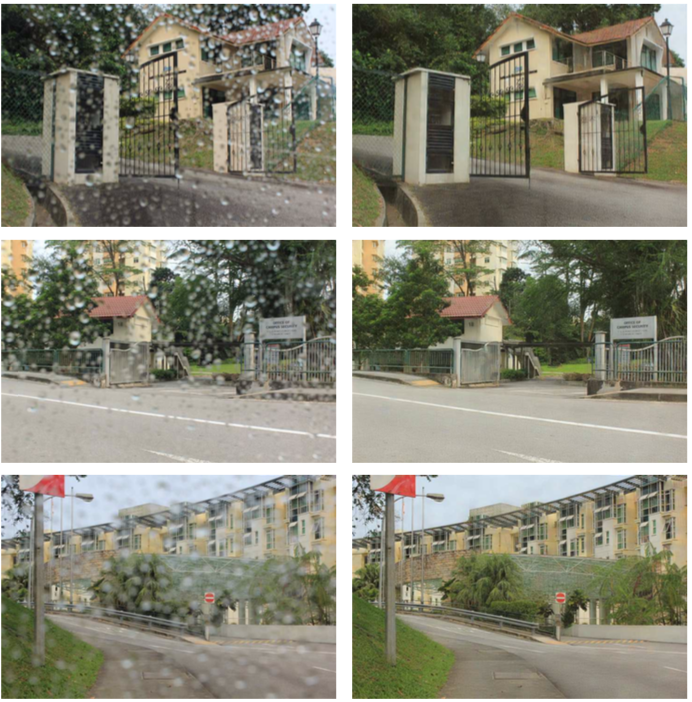
\includegraphics[width=0.75\textwidth]{figure/attention_gan_example.png}
		\caption{去除图像中的雨滴~\cite{qian2018attentive}}
		\label{subfig:attention_gan}
	\end{subfigure}
	\begin{subfigure}{0.45\textwidth}
		\centering
		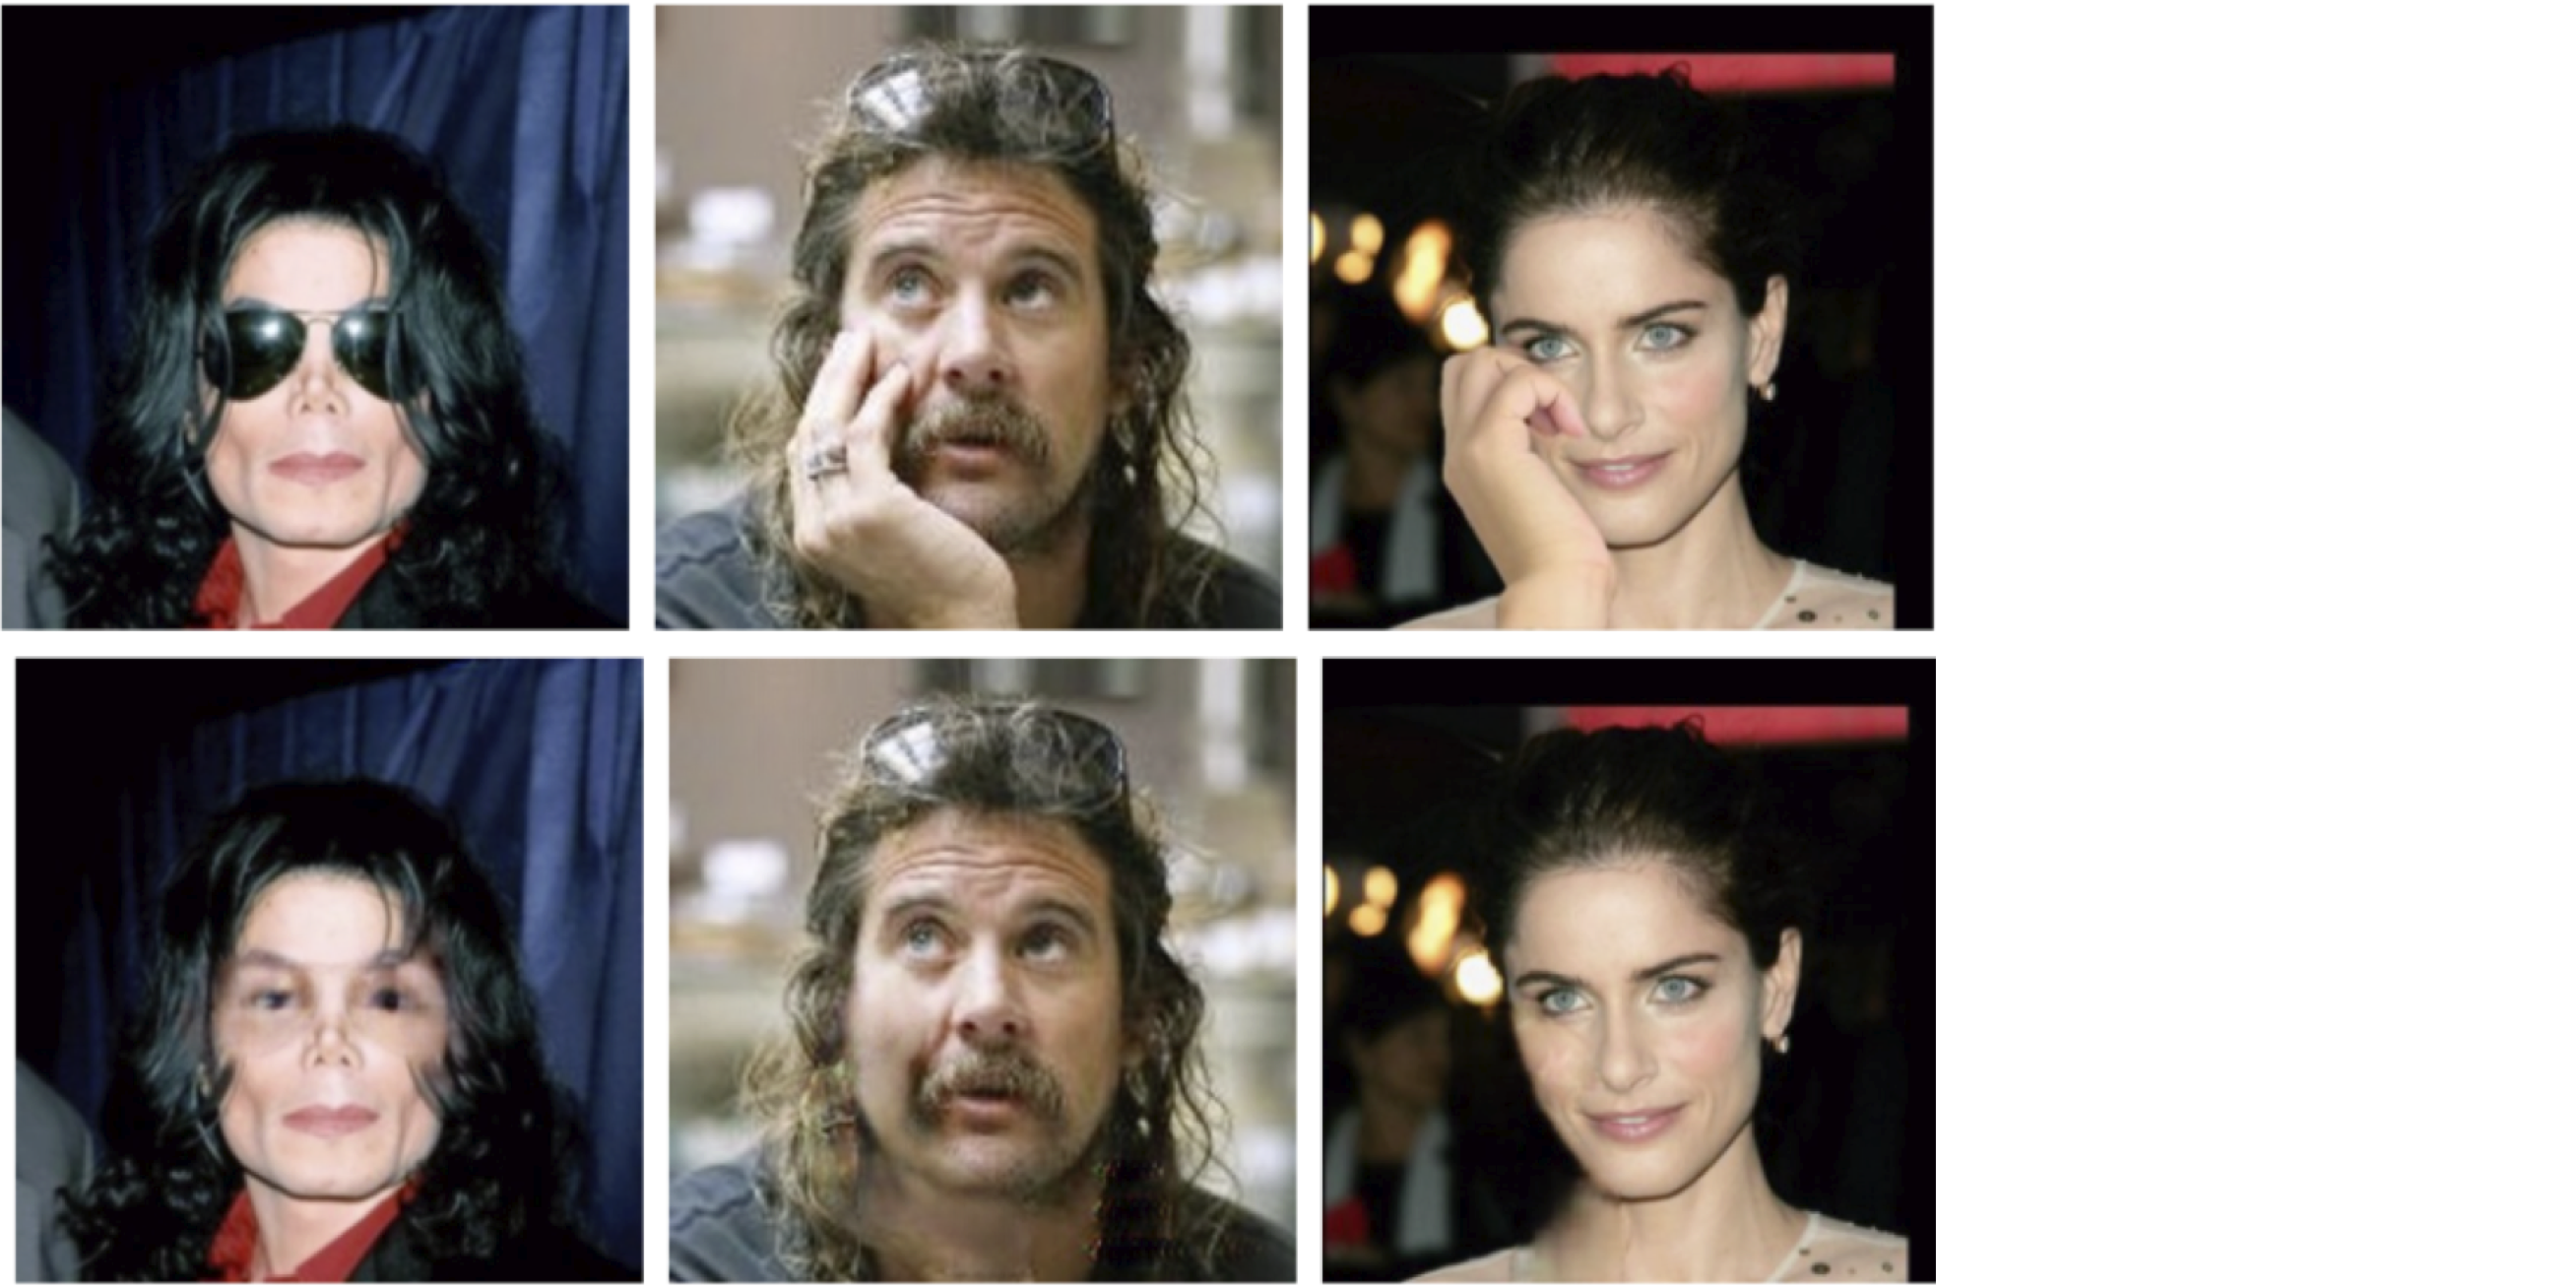
\includegraphics[width=1.5\textwidth]{figure/face_de_occulusion.png}
		\caption{去除人脸中的遮挡物~\cite{yuan2019face}}
		\label{subfig:face_de_occulusion}
	\end{subfigure}
	\caption{GAN去除图像遮挡物示例(图片均来自于对应原文~\cite{qian2018attentive,yuan2019face})}
	\label{mul_fig:gan_auto_encoder_example}
\end{figure}


%\paragraph{解决思路} 面对弱监督条件下,疾病标记物的精确定位这一问题,鉴于已有方法只能粗略定位到疾病标记物,我们最先想到用图像生成即对抗生成网络的思路去做,并且输入输出图像尺寸相等,这样就避免了CAM和Grad-CAM中由于上采样所造成的定位不精确的问题。如果用映射$H$来表示生成器,给定输入图片$I^{h\times w\times d}$(图像的高、宽和深度分别为$h$,$w$,$d$),则$H$是一个图像到图像的映射,可形式化为:
%\begin{equation*}
%H: I \to I'.
%\end{equation*}
%其中$I'^{h\times w\times d}$与$I$一样,均表示一张图像。假设生成器有识别疾病标记物或者说患病区域的能力,不难想象,在理想状态下,给定输入图像$I$,生成器给出其输出图像$I'$,根据输入图像类别是正常还是异常,有以下推断:

%\noindent 1)如果输入图像$I$是正常图像,则可认为输出图像$I'$与输入图像$I$一致,即此时输入图像并没有像素强度发生改变。

%\noindent 2)如果输入图像$I$是异常图像,可以想象,与输出图像$I'$相比,输入图像$I$中只有极少数像素强度发生改变,而绝大部分像素强度没有发生改变,那么我们完全有理由认为这些发生改变了的像素便是疾病标记物,此时我们可以认为输出图像$I'$是异常输入图像$I$去除疾病标记物的“正常”版本,且疾病标记物的准确位置$Y$为:
%\begin{equation}\label{equ:idea}
%Y=|I'-I|=|H(I) - I|.
%\end{equation}
%\noindent 根据等式\ref{equ:idea},一旦得到这样的生成器,便可以实现疾病标记物的精确定位。根据以上设计,可知生成器满足以下两个条件:
%\begin{itemize}\label{item:satified_conditions}
%	\item 给定输入图像$I$,生成器能生成具有与输入图像大小相同的输出图像$I'$。 
%	\item 生成器具有良好的识别疾病标记物的能力。
%\end{itemize}
%\noindent 对于条件一,实现比较容易,全卷积网络或者编码器-解码器,都能满足这一条件。考虑到近些年来编码器-解码器在图像生成领域所取得的巨大成就,我们优先考虑选择编码器-解码器。主要难点在于第二点:如何让编码器-解码器具备识别疾病标记物或者说异常信号的能力。编码器-解码器作为一种无监督模型,最朴素的想法是只使用正常图像训练编码器-解码器,使其具有重建正常图像或者说正常信号的能力,当送入异常图像时,由于编码器-解码器并未见过异常信号,故编码器-解码器无法较好重建异常信号,从而间接使编码器-解码器具有识别异常信号的能力。实际上,在单张图像中,由于疾病标记物所占的像素在整张图像中只占很小一部分($\le 2\%$),再加上CNN强大的拟合能力和高容量,这种位于局部的图像细节差异往往非常不明显,很难被凸显出来。因此,需要引入其他模块来指导编码器-解码器,在弱监督条件下,图像级标签是有提供的,故可引入一个CNN分类器。根据以上设计(参见\ref{item:satified_conditions}小节中编码器-解码器满足的两个条件),如果编码器-解码器具备识别疾病标记物的能力,对于异常图像$I_{lesion}$和正常图像$I_{normal}$,在理想情况下,有:
%\begin{itemize}\label{ite:ideal_situation}
%	\item 对于输入图像$I_{lesion}$,输出图像$({H}(I_{lesion}))$与原输入图像比只有极少数像素强度发生改变,是其“正常”版本,故$({H}(I_{lesion})-I_{lesion})$仍含有原始图像$I_{lesion}$上的全部疾病标记物。 
%	\item 对于输入图像$I_{normal}$,输出图像${H}(I_{lesion})$与原输入图像比未发生像素强度的改变,仍为正常图像,故$({H}(I_{normal})-I_{normal})$不含有任何疾病标记物。
%\end{itemize}
%我们可以发现,对于输入图像$I$,无论$I$是正常图像还是异常图像,编码器-解码器的输出图像与输入图像之差$({H}(I)-I)$与原始图像$I$的标签是一致的,故我们可以试图通过引入一个CNN分类器完成一个分类任务来使编码器-解码器具备识别疾病标记物的能力,只是CNN分类器的输入不再是原始输入图像$I$,而是编码器-解码器的输出图像和原始输入图像之差,这样的取差操作还有一个好处是可以排除原始图像中无关信息(如背景)的干扰,让CNN分类器更加关注与疾病标记物相关的信息。此时的模型是编码器-解码器和CNN分类器的组合。但是,考虑到CNN分类器在做分类任务时,由于卷积操作感受野的局部性,CNN分类器可能是根据图像中最为突出、最为重要的图像模式或者特征进行分类的,比如说,一张图像中有很多只猫,固然CNN分类器能够正确完成分类,但是其分类依据极有可能是在图像中所占比例最大、毛色最突出的某一只或某几只猫,而没有考虑到甚至直接忽略在图像的某一角还有一只甚至几只相对不够突出的猫,这种情况在含有多个大小不一的目标物体的图像中是很有可能发生的。同理,如果一张医学图像$I_{lesion}$中含有多个大小不一、形状各异、分布广泛的疾病标记物,而编码器-解码器只有部分识别疾病标记物的能力,则其输入图像$I'_{lesion}$很可能只有部分相对不够明显的疾病标记物,则此时输出图像和输入图像的差$(I'_{lesion}-I_{lesion})$中只有相对比较明显的疾病标记物,显而易见,这种情况是能够骗过CNN分类器,使其作出此输入为异常的判断。注意,此时$(I'_{lesion}-I_{lesion})$只能定位到相对较为明显的疾病标记物而漏掉了相对不够明显的疾病标记物。显然,我们还需要更为精确的定位结果。

%鉴于以上情况,考虑到对抗生成网络与编码器-解码器的有效结合并在图像中能较好去除遮挡物,如去除单张图像中的雨滴~\cite{qian2018attentive}(见图\ref{subfig:attention_gan}),去除人脸中的遮挡物~\cite{yuan2019face}(见图\ref{subfig:face_de_occulusion})。尤其是对于雨滴这种相对较小、分布较为广泛的物体仍能处理的相当好,完全有理由考虑再引入对抗生成网络进一步帮助编码器-解码器去除图像中相对不够明显的疾病标记物。如果将编码器-解码器看做对抗生成网络中的生成器,那么只需额外引入一个判别器模块即可。此时,我们提出的模型由编码器-解码器、CNN分类器和判别器组成,其中,判别器和生成器共同组成了对抗生成网络。更多的模块引入,也就意味着需要更为精巧的组合方式和训练方式。接下来,本文\ref{sec:model_architecture_intro}小节将详细介绍整体模型结构和每个模块的模型结构。

%\begin{figure}[h!]
%	\begin{subfigure}{0.45\textwidth}
%		\centering
%		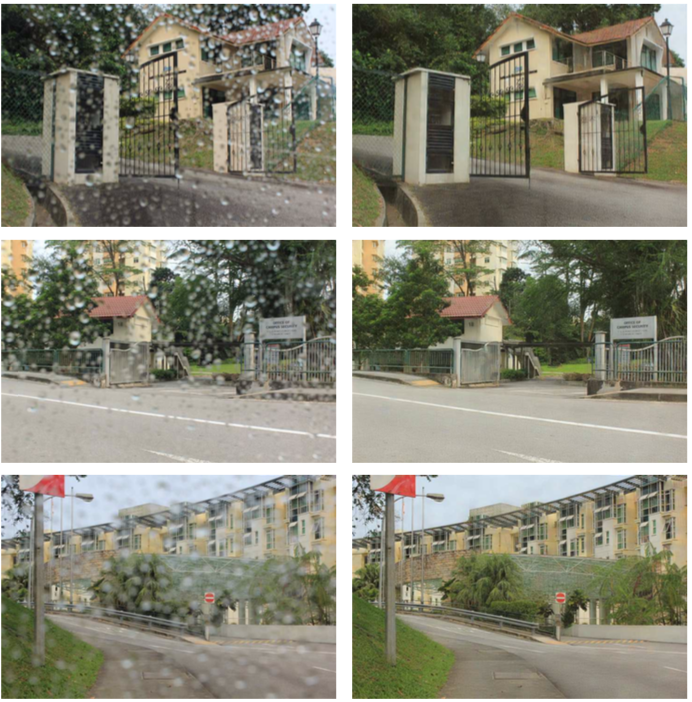
\includegraphics[width=0.75\textwidth]{figure/attention_gan_example.png}
%		\caption{去除单张图像中的雨滴(图片来自于原文)。}
%		\label{subfig:attention_gan}
%	\end{subfigure}
%	\begin{subfigure}{0.45\textwidth}
%		\centering
%		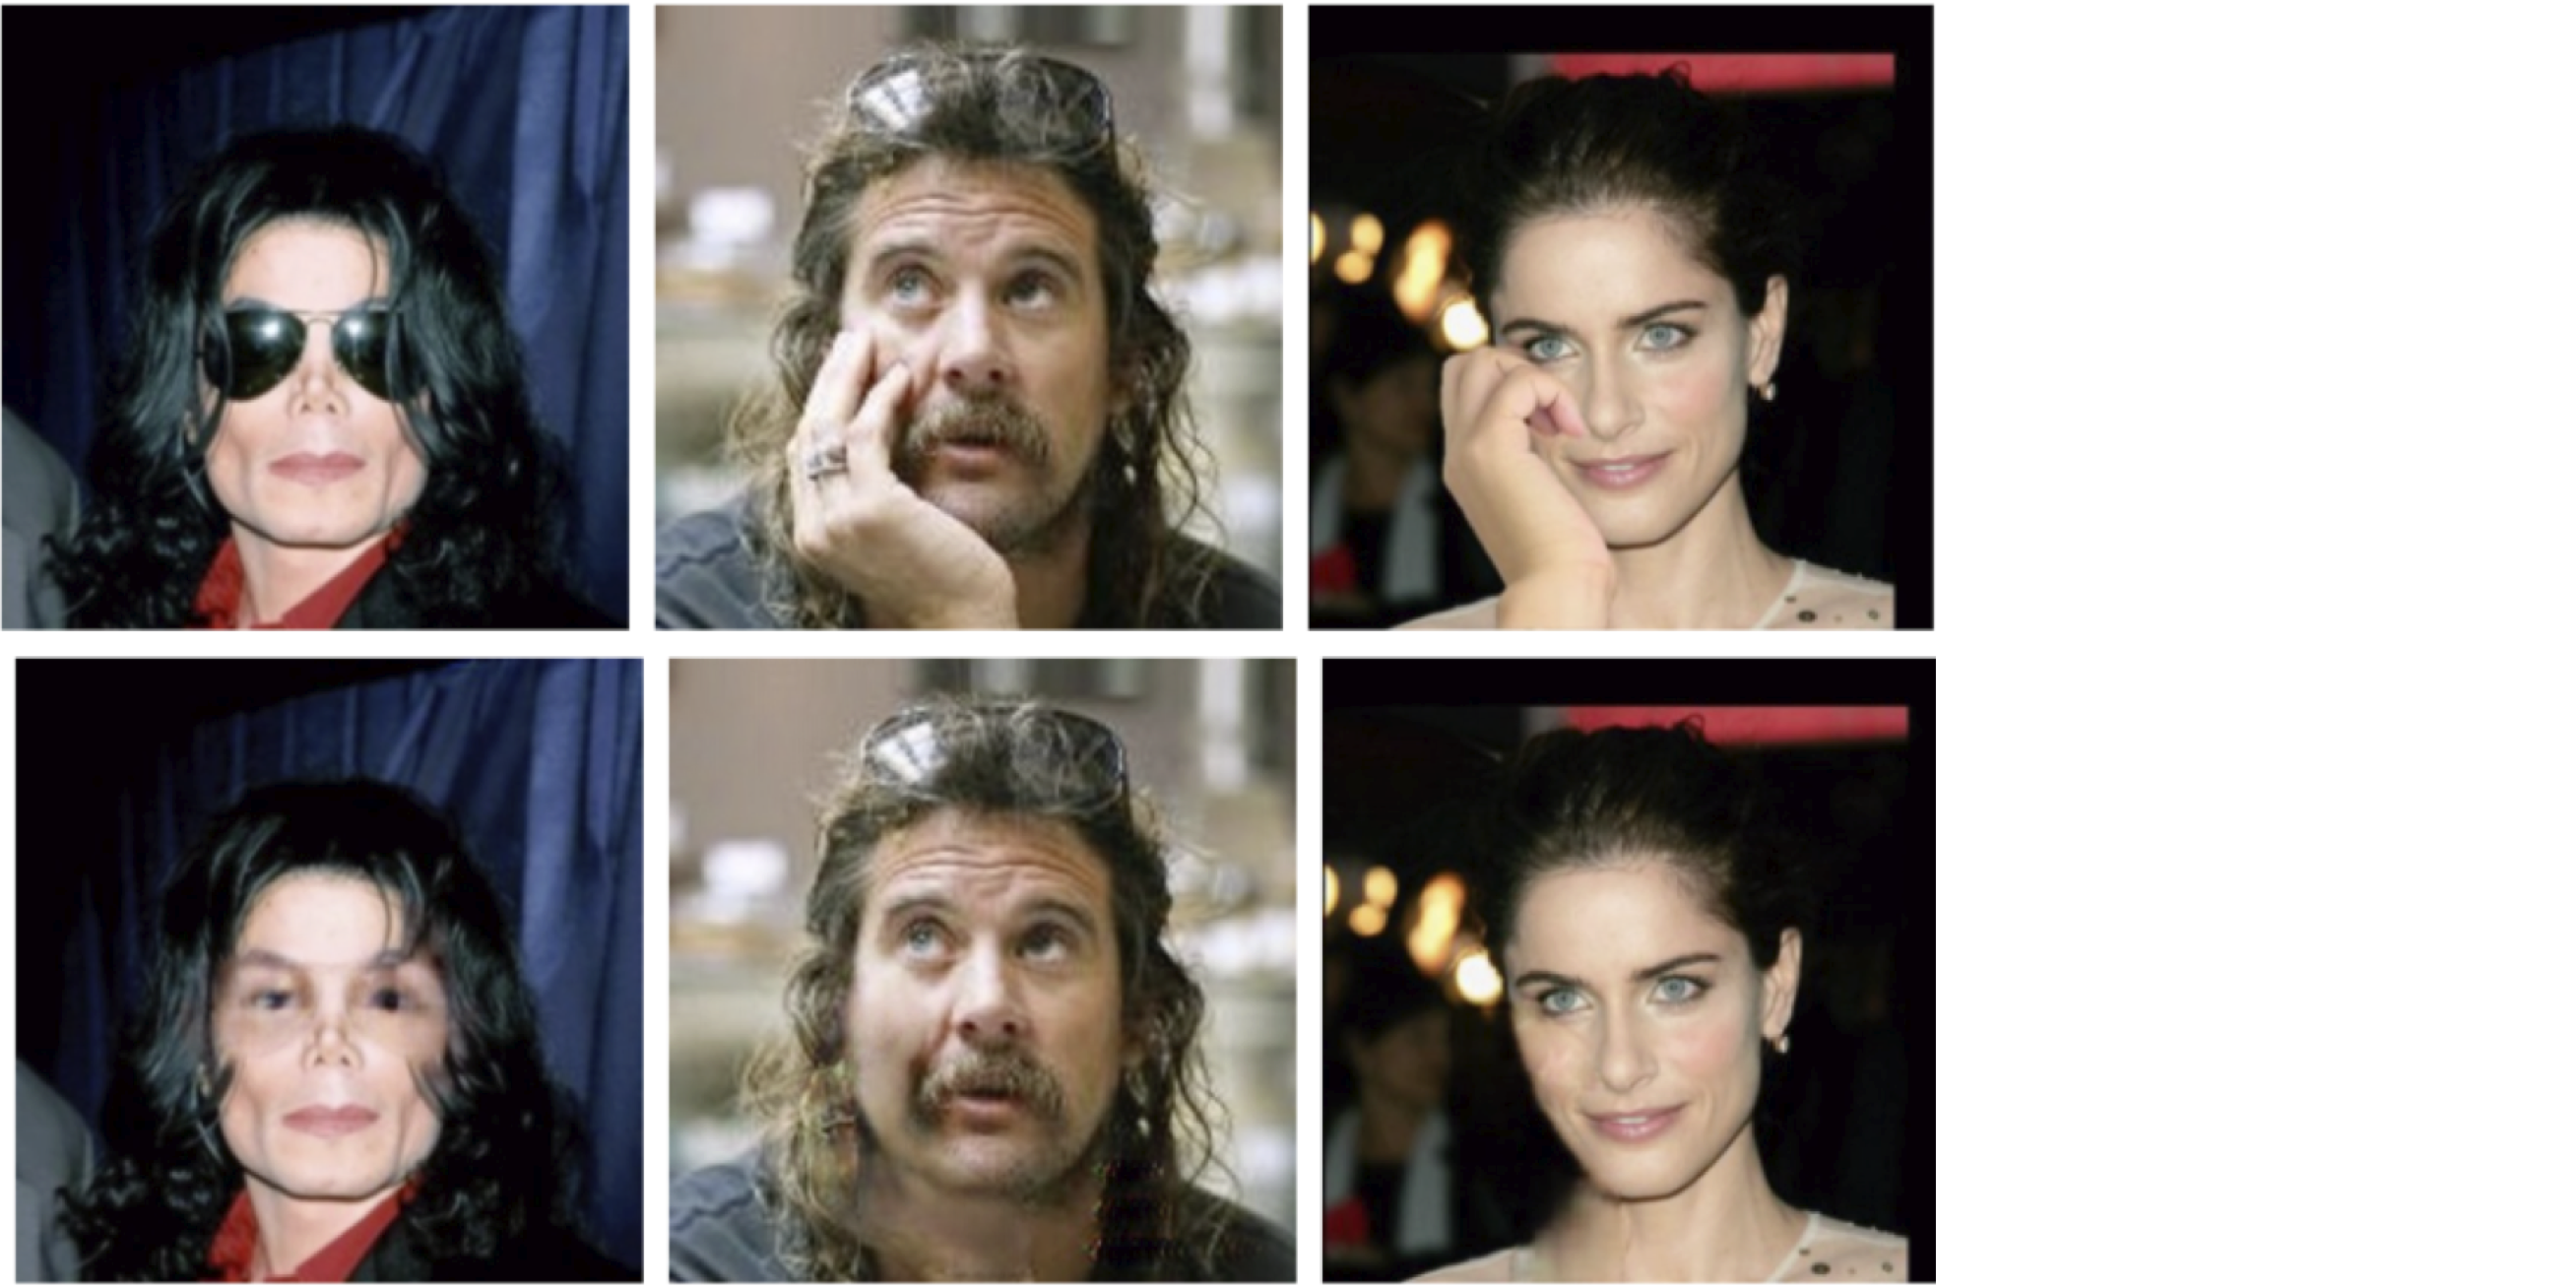
\includegraphics[width=1.5\textwidth]{figure/face_de_occulusion.png}
%		\caption{去除人脸中的遮挡物(图片来自于原文)。}
%		\label{subfig:face_de_occulusion}
%	\end{subfigure}
%	\caption{对抗生成网络与编码器-解码器的有效结合并在图像中能较好去除遮挡物示例。}
%	\label{mul_fig:gan_auto_encoder_example}
%\end{figure}

\section{模型结构介绍}\label{sec:model_architecture_intro}
在\ref{sec:idea_thinking}小节中,本文已经介绍了解决疾病标记物的解决思路和理论建模。本小节内容将详细介绍整体模型结构和各个子模块模型结构,力求读者能清晰明了理解本文方法的核心思想。

%具体来说,本文将在\ref{subsec:model_architecture}小节中详细介绍整体模型结构及各个子模块在整体模型中所起到的作用和相互关系。接下来,在\ref{subsec:encoder_decoder_model}小节、\ref{subsec:cnn_classifier_model}小节和\ref{subsec:discrimintor_model}小节分别介绍编码器-解码器、CNN分类器和判别器的模型结构。下面展开相关内容的具体阐述。

\subsection{模型结构介绍}\label{subsec:model_architecture}
本文提出的模型目的是在仅图像级别的标签可用时,精确定位异常图像中潜在的生物标志物或病变区域。我们的想法是设计一种可以学会直接查找疾病标记物的新架构。出于这种动机,我们提出了一种新颖的深度神经网络。这种网络结合了两种不同的学习架构(见图\ref{fig:our_model_architecture}):发挥监督作用的CNN分类器和负责图像生成的GAN(由编码器-解码器和判别器组成)。CNN分类器和判别器可以共同帮助编码器-解码器更有效地从输入图像中除去疾病标记物。训练完成后,可以通过编码器-解码器的输入中减去其输出来定位疾病标记物。
\begin{figure}[h]
	\centering
	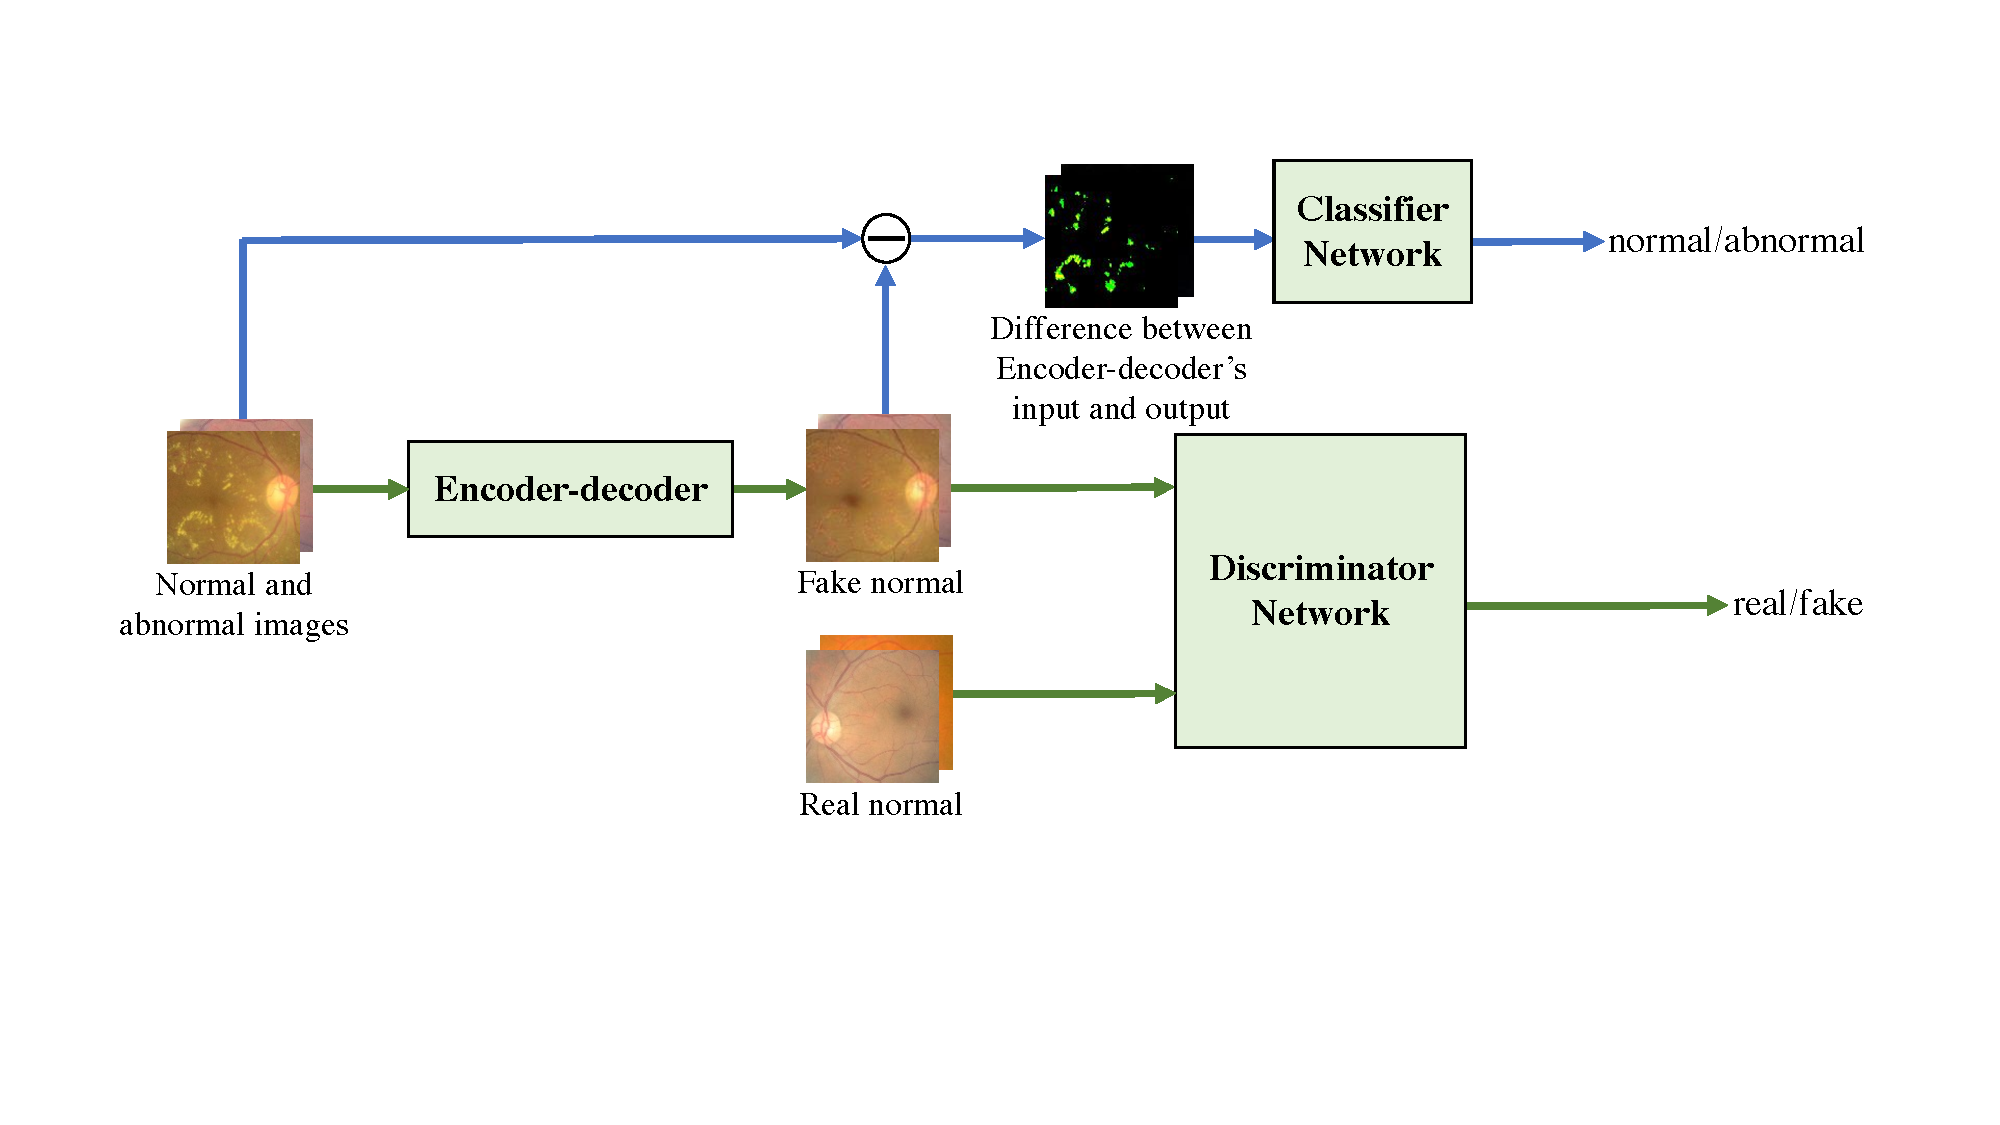
\includegraphics[width=1.0\textwidth]{figure/method.pdf}
	\caption{本文提出的疾病标记物定位网络} 
	\label{fig:our_model_architecture}
\end{figure}
在提出的体系结构中,编码器-解码器网络尝试从输入图像中删除任何潜在的生物标记,为异常的输入图像生成伪造的正常图像,或者在输入正常的情况下将输出图像与输入保持相同。通过从其输入中减去编码器-解码器的输出,可以轻松地对任何疾病标记物进行定位和分析。尽管可以仅使用正常图像来训练这种编码器-解码器,但这并没有利用现有的异常图像,因此不能直接学习生物标记特征以进行定位。取而代之的是,为了更有效地实现编码器-解码器的目标,在编码器-解码器的顶部添加了CNN分类器,其中输入是从其输入中减去编码器-解码器的输出,而期望的输出是原始输入图像的标签。为了准确地对图像进行分类,CNN分类器与编码器-解码器必须将异常图像与正常图像区分开。理想情况下,如果分类器的输入仅包含异常原始图像的生物标记,而对于正常图像则不包含任何生物标记(各处均为零),则分类器将更容易,也更准确地预测原始图像的类别。换句话说,训练更准确的分类器可以帮助编码器-解码器的输出保持正常区域,并从原始图像中移除疾病标记物,从而使分类器的输入仅包含疾病标记物的信号。

但是,分类器可能会帮助仅从原始输入图像中定位部分生物标记。这是因为定位来自原始异常图像的部分生物标记信号(以及定位来自正常图像的信号很少)足以使分类器轻松区分正常图像和异常图像。在这种情况下,编码器-解码器输出仍将包含一些生物标记。

为了进一步帮助编码器-解码器从原始(异常)图像中删除潜在的生物标记,添加了一个鉴别器来判断编码器-解码器的输出是否看起来像真实的正常图像。 通过强制编码器-解码器的输出看起来更像正常图像,鉴别器帮助编码器-解码器从原始图像中去除尽可能多的生物标记信号。

显然,编码器-解码器和鉴别器一起形成了生成对抗网络。读者可能会认为,在架构中没有分类器组件的对抗生成网络本身足以帮助编码器-解码器从图像中删除潜在的生物标记。但是,对抗生成网络本身可能会提供过多帮助,以至于尽管编码解码器生成的图像非常正常,但与输入相比,编码器解码器输出的正常区域也可能会发生变化。在这种情况下,编码器-解码器的输出与其输入(即分类器的输入)相减会同时包含正常信号和生物标记信号,这又使分类器将异常图像与正常图像区分开来相对较困难。这意味着分类器和鉴别器应该一起工作以帮助编码器-解码器去除潜在的生物标记,即鉴别器帮助编码器-解码器输出正常图像,而分类器帮助编码器-解码器仅改变生物标记区域以生成正常输出。在实验也已经证实了这一点(参见第\ref{sec:experiments}相关章节)。

\subsection{编码器-解码器模块}\label{subsec:encoder_decoder_model}
\ref{subsec:model_architecture}小节中阐述了整体模型及各个子模块各自的作用,接下来进行子模块的介绍。本文决定选用在U-Net的基础上进行结构或者模块的微调,进而将U-Net迁移到本任务上来。原因主要有以下三点:
\begin{figure}[h]
	\centering
	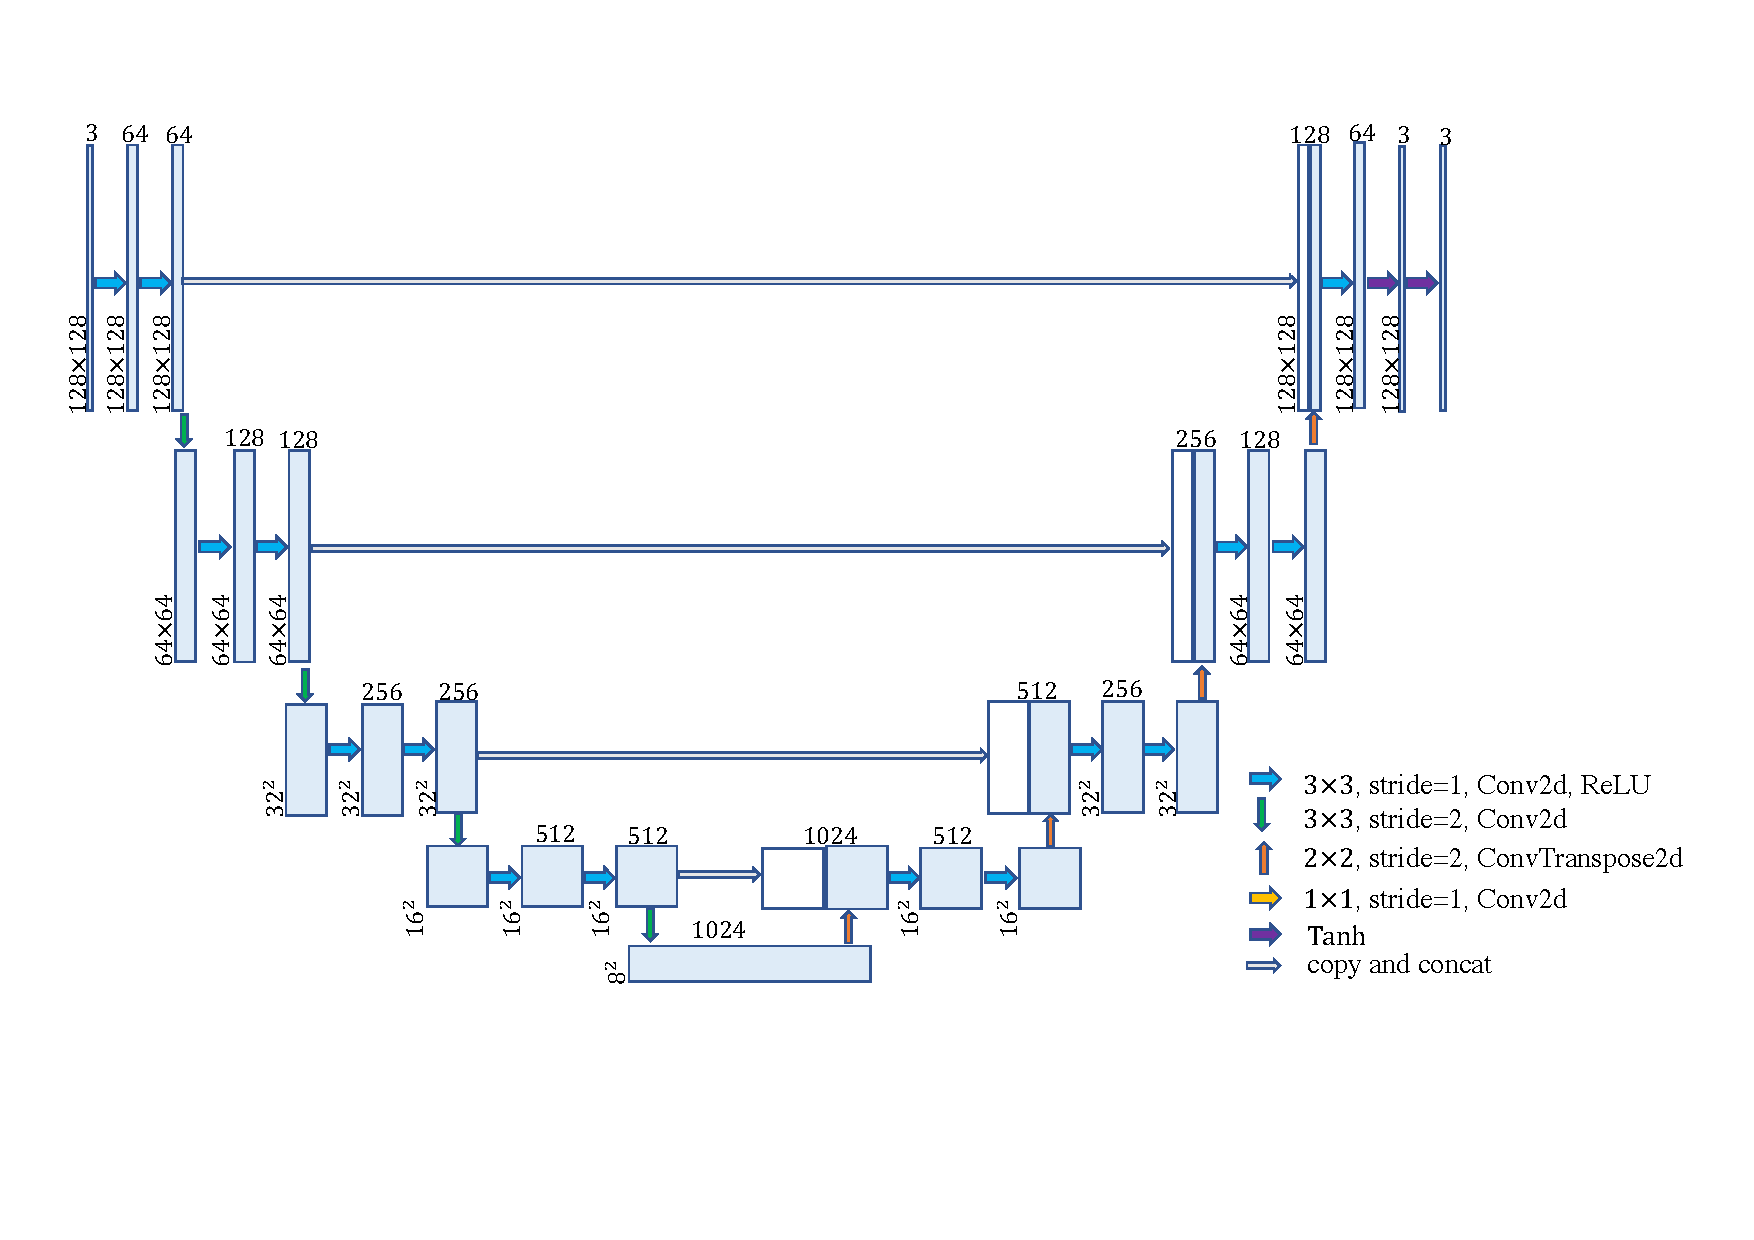
\includegraphics[width=1.0\textwidth]{figure/auto_encoder_architecture}
	\caption{本文编码器-解码器模块}
	\label{fig:auto_encoder_architecture}
\end{figure}
\begin{itemize}
	\item 近些年来,U-Net在医学影像分析领域应用越来越广泛,无论是在处理医学分割上~\cite{oktay2018attention, dong2017automatic, zhang2018ct},还是在把U-Net当做生成器与其他判别器来组成对抗生成网络上,都表现不俗,性能出色。
	\item 在疾病标记物的精确定位任务中,只需要极少像素强度发生改变,而其他绝大部分像素都需要较好的重建出来,而U-Net的跨层结构能够很好的将编码阶段的特征图融合到解码阶段,有利于图像尤其是具有丰富细节纹理的图像的重建。对于眼底图像(见图\ref{fig:biomarker_localization_example})的重建来说有重大意义。
	\item U-Net是全卷积网络的一种,可允许任意尺寸大小的图像输入,这增加了输入图像尺寸大小的灵活,上采样的倍数也可由U-Net的深度灵活控制。另外,由于跨层的存在,使得梯度回传比较容易,不容易出现梯度消失情况。
\end{itemize}
因此,本文选用U-Net为基本结构,将U-Net迁移到本文任务上来。与原始U-Net相比,本文在模型结构上最终做了如下调整:
\begin{itemize}
	\item 在编码阶段,为了减少在下采样过程中造成的信息丢失,本文采用的编码器-解码器中使用卷积(卷积核大小为$3\times 3$,步长为2)代替最大池化层。相应地,在解码阶段,编码器-解码器中使用反卷积(卷积核大小为$2\times 2$,步长为2)代替上采样操作。
	\item 由于编码器-解码器的输入图像经过预处理之后的范围为$[-1,1]$,在解码阶段的$1\times 1$卷积之后,编码器-解码器使用Tanh激活函数替代了Sigmod激活函数。
\end{itemize}
经过以上微调之后,编码器-解码器的最终模型结构如图\ref{fig:auto_encoder_architecture}所示,图中输入图像尺寸为$128\times 128$,网络深度为5。可以看出,编码器-解码器还是以U-Net为骨架,编码阶段和解码阶段在网络结构上呈现“U”形。网络中每一层由2个卷积层组成。在编码阶段,随着深度的增加,特征图尺寸逐步减小,特征图数量或者说卷积核数量逐渐增加,直到到达最底层。与编码阶段相反,解码阶段随着深度的较少,特征图尺寸逐步增大,特征图数量或者卷积核数量逐渐减小,同时来自编码阶段的特征不断通过跨层被融合到解码阶段的高层特征中,直到到达最顶层。
\subsection{CNN分类器模块}\label{subsec:cnn_classifier_model}
CNN分类器主要考虑的问题是如何选择一个较为优秀的分类网络,最终选择使用ResNet-18~\cite{he2016deep}。一方面,ResNet系列网络具有良好的特性。而编码器-解码器深度也较深,采用ResNet网络有利用避免梯度消失(相关数学原理解释见\ref{subsec:cnn_introduction}小节)。另一方面,ResNet网络相对于VGG~\cite{simonyan2014very}等网络,参数量较少,计算开销较小。而相对于DenseNet~\cite{huang2017densely}、Inception~\cite{Szegedy2015RethinkingTI}等网络,ResNet模型结构较为简单,易于理解。CNN分类器的模型结构如图\ref{fig:classifier_architecture}所示,可以发现,CNN分类器没有对原始ResNet-18进行较大改变,只是在残差模块之前,用$3\times 3$卷积代替了原始$7\times 7$卷积。这主要是因为原始ResNet-18针对输入尺寸$224\times 224$的图像,而CNN分类器针对输入尺寸$128\times 128$的图像。
\begin{figure}[h]
	\centering
	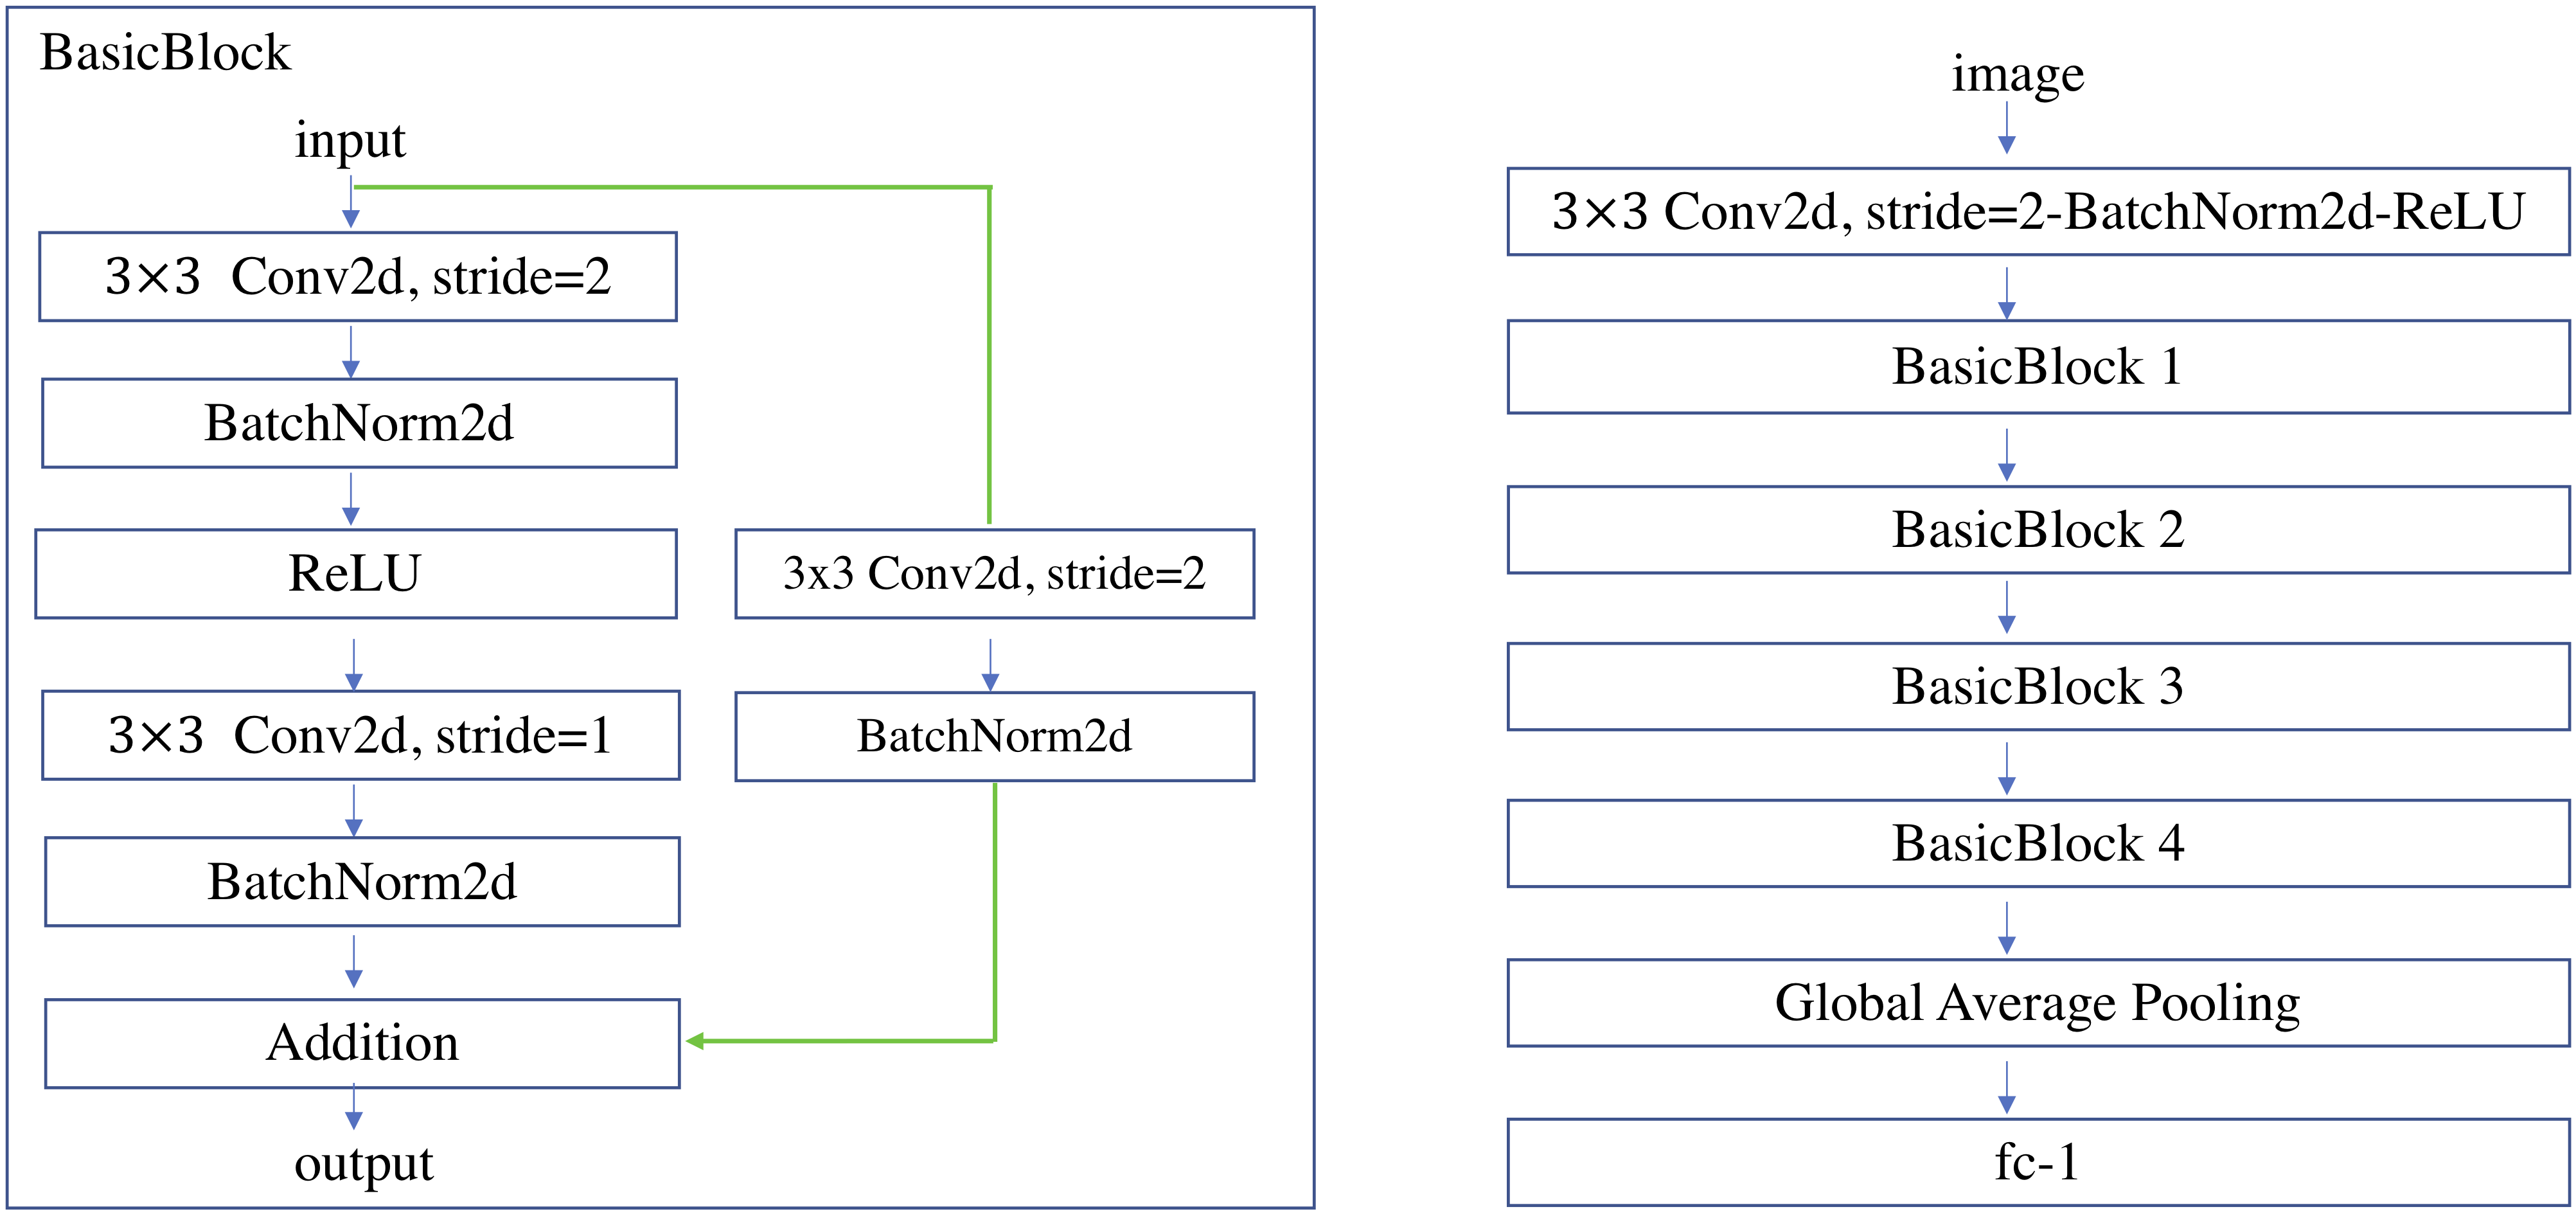
\includegraphics[width=1.0\textwidth]{figure/classifier_architecture.png}
	\caption{本文CNN分类器模块}
	\label{fig:classifier_architecture}
\end{figure}
\subsection{判别器模块}\label{subsec:discrimintor_model}
本小节将详细介绍本文判别器的模型结构。如图\ref{fig:discrimintor_architecture}所示,判别器模块基本单元由卷积操作(卷积核大小为$3\times 3$)、BatchNormalization~\cite{ioffe2015batch}和Leaky ReLU激活函数(负斜率为0.2)~\cite{maas2013rectifier}组成。不同的是,在下采样阶段(图\ref{fig:discrimintor_architecture}中的DownConv2d单元),采用步长为2的卷积,从而达到下采样的目的,同时随着中的DownConv2d单元的增加,卷积核的数量也以2倍关系增长(卷积核数量基数为64);而在精细化提取特征阶段(图\ref{fig:discrimintor_architecture}中的Conv2dBloc单元),卷积操作的步长为1,特征图尺寸不会发生变化,同时在此阶段卷积核数量也不发生任何改变。另外,网络深度可由DownConv2d单元和Conv2dBlock单元来共同控制。最后,将第一个DownConv2d单元的特征输出、最后一个DownConv2d单元的特征输出以及最后一个Conv2dBlock单元的特征输出在经过全局均值池化层之后进行拼接操作,完成低分辨率但语义强的特征(最后一个Conv2dBlock单元的特征输出)和高分辨率但语义弱(第一个DownConv2d单元的特征输出和最后一个DownConv2d单元的特征输出)的特征结的相互融合,最后送入全连接层,输出对输入图像是否是编码器-解码器生成的置信度分数。

\begin{figure}[h]
	\centering
	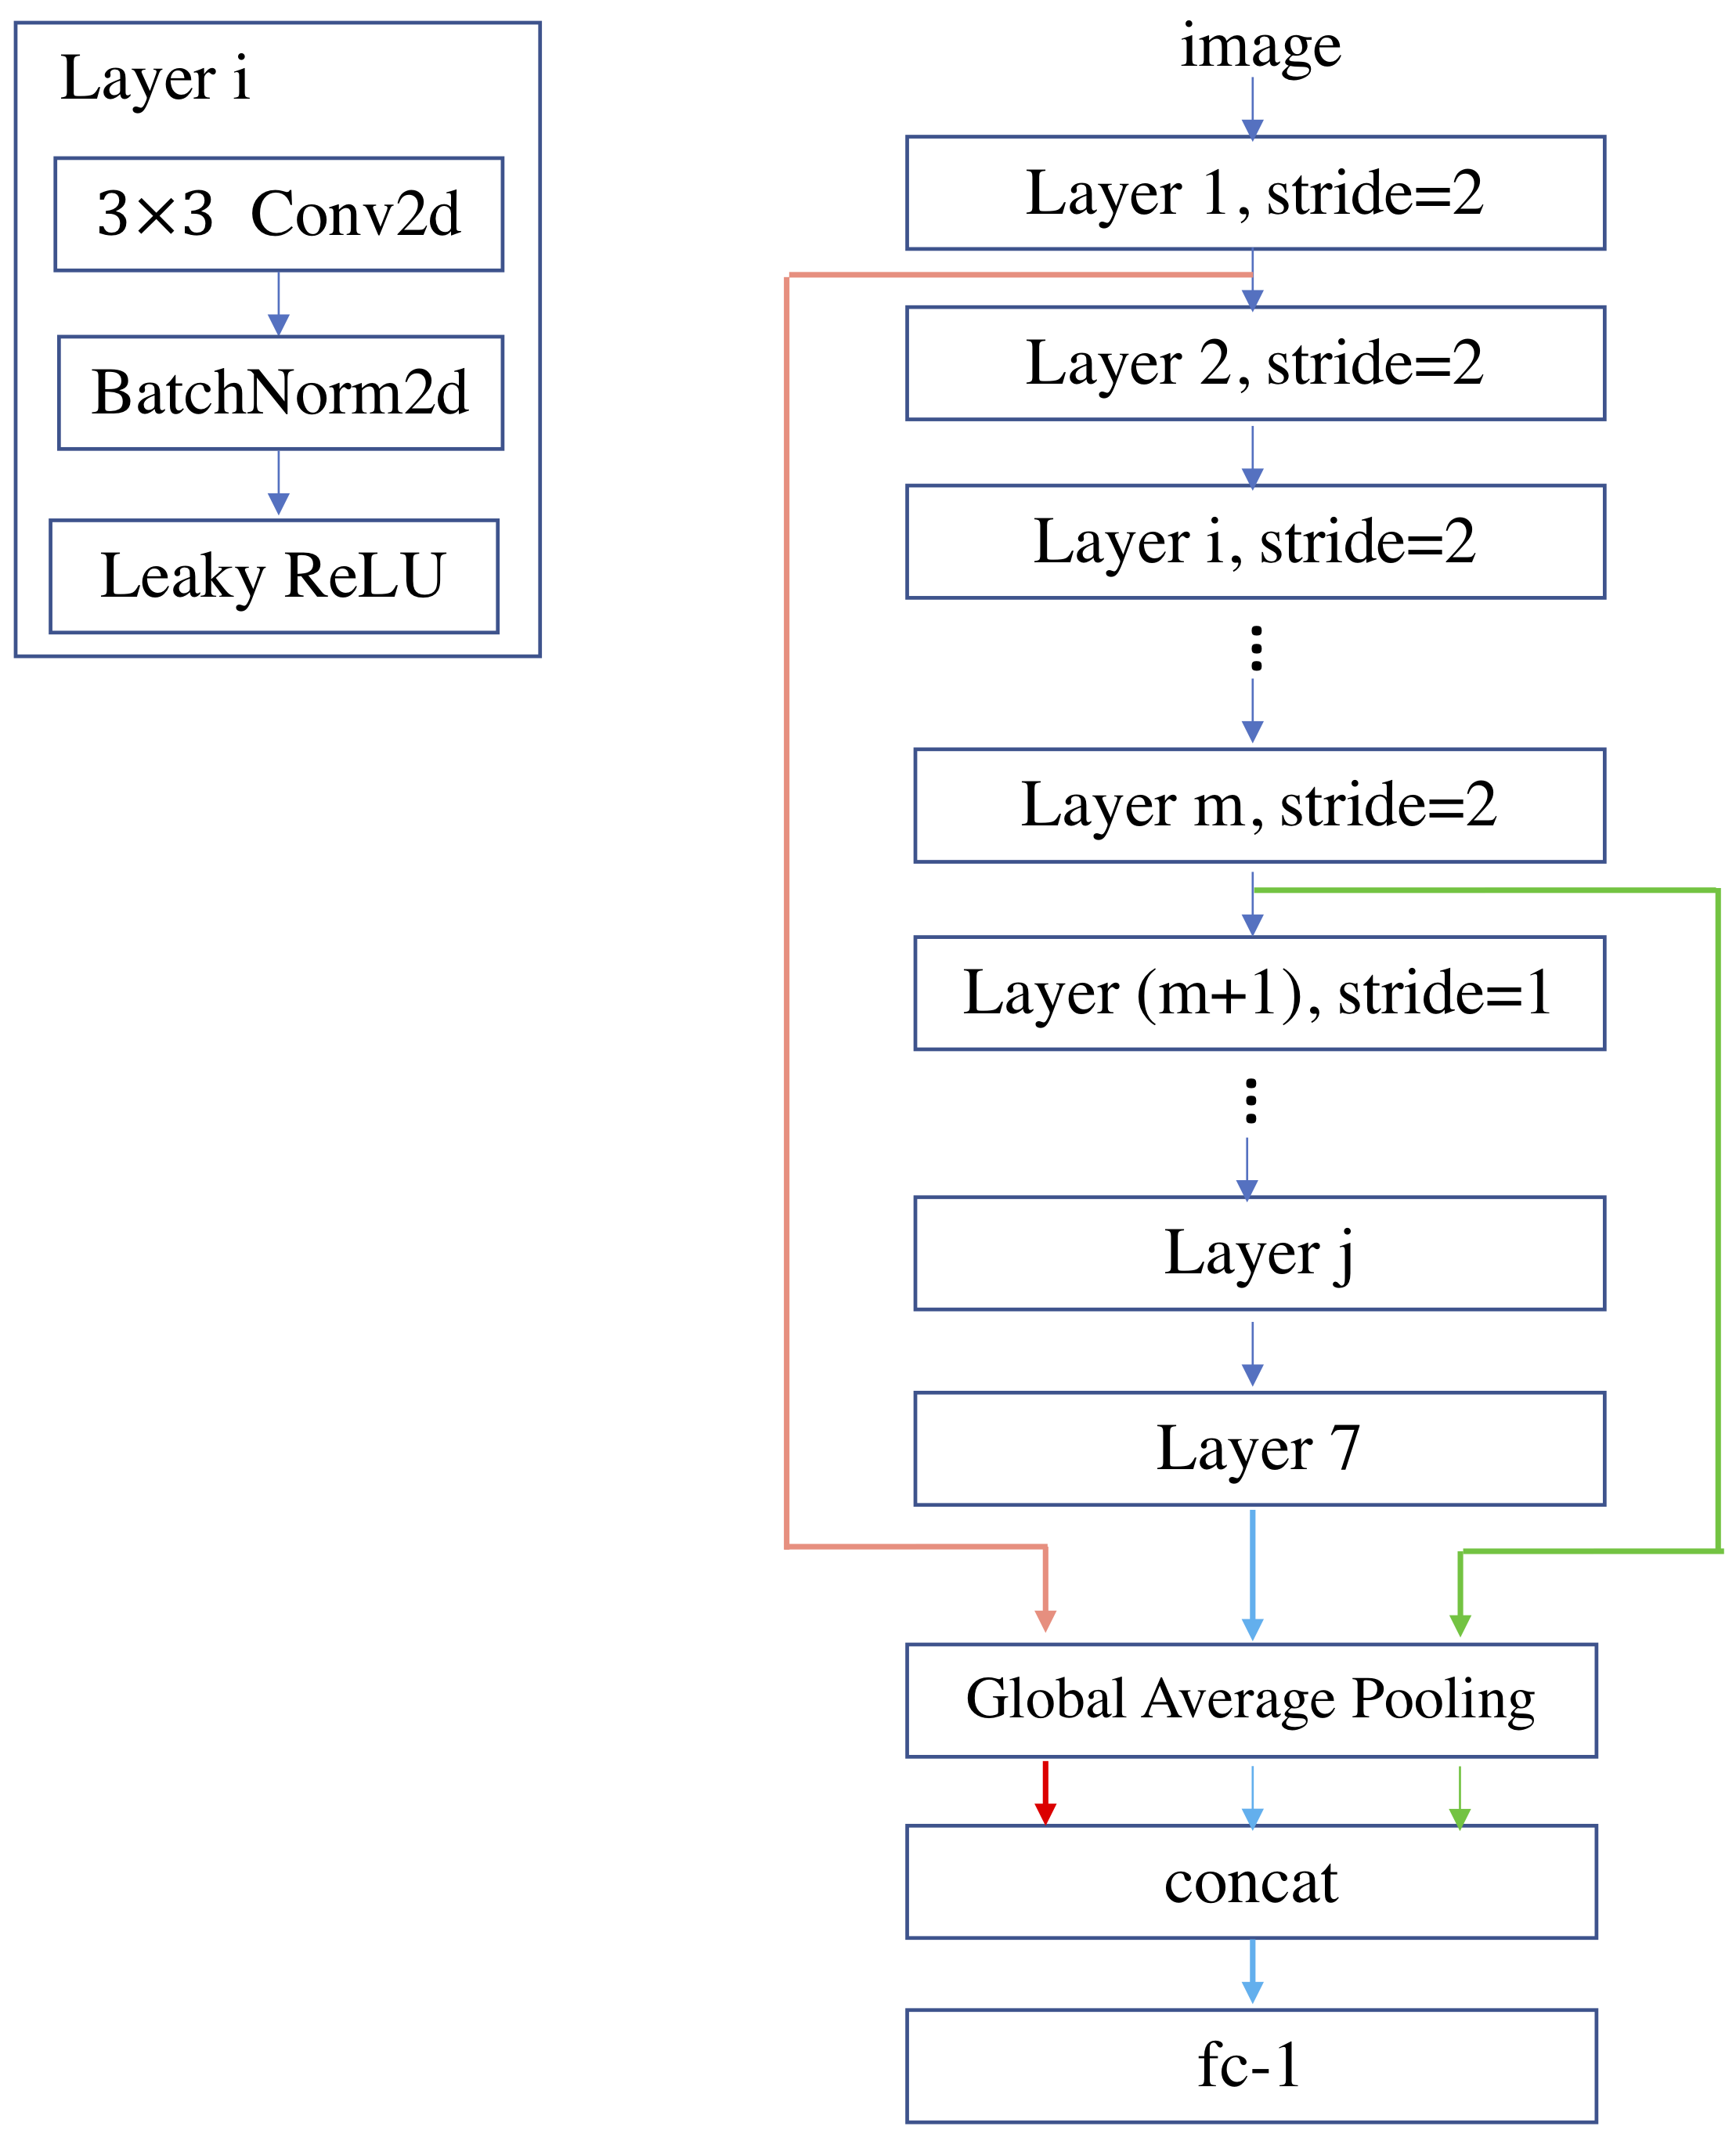
\includegraphics[width=1.0\textwidth]{figure/discrimintor_architecture.png}
	\caption{本文判别器模块}
	\label{fig:discrimintor_architecture}
\end{figure}

本文参考了特征金字塔~\cite{lin2017feature},判别器模块和与普通CNN判别器相比,最主要的改动是增加了跨层结构。该结构通过从上而下的路径连接,来将低分辨率但语义强的特征和高分辨率但语义弱的特征结合起来,使得原图像中的丰富细节信息比如纹理信息都能被捕捉到。换句话说,就是使用内网倒特征金字塔(特征图尺寸从上到下依次减小)取代特征化图像倒金字塔(随着卷积的堆叠,特征图尺寸依然是从上到下依次减小),且没有牺牲表示能力,速度和内存。这种设计最初用于解决物体检测中小物体在连续特征图的下采样过程中容易被忽略的问题。由于浅层高分辨率但语义弱的特征中往往包含了小物体的信息,故可通过多尺度特征图的融合,可以将这些小物体的特征直接送到高层,与低分辨率但语义强的特征结合起来,使得各种大小不一的物体都能被CNN检测到。而医学影像中的疾病标记物也有这种特点,具体来说,疾病标记物的形状通常是不确定的,大小各异,并且数量往往不是一个,而是多个。因此,如果对这些大小不一的疾病标记物进行比较,也会发现有些疾病标记物属于大物体或者说大目标,而另外一些疾病标记物属于小物体或者说小目标,甚至还会存在一些人类甚至专业医生都难以察觉到的微小疾病标记物。也就说,这种在物体检测问题中出现的小物体难以发现的难题在医学影像领域的疾病标记物定位问题中不光存在,而且更加突出。这也是本文判别器模型中加入跨层结构的必要性所在。

在上文提到的诸多GAN中,训练WGAN-GP时梯度相对比较稳定,不易发生梯度消失,Wasserstein-1距离对训练过程也有指示作用,故本文选用WGAN-GP~\cite{gulrajani2017improved}。注意,此时判别器不再是二分类器,而是去拟合Wasserstein-1距离的回归器,该任务属于回归任务,故最后一层全连接层之后也没有Sigmoid激活函数。

\section{训练策略与损失函数}\label{sec:loss_func_training_stragies}
在\ref{sec:model_architecture_intro}小节中,本文介绍了本题提出方法的模型结构以及各个子模块所起的作用。本节内容将在此基础上进一步介绍训练模型时的训练策略(见\ref{subsec:traing_stragies}小节)以及损失函数(见\ref{subsec:loss_func}小节)。
\subsection{训练策略}\label{subsec:traing_stragies}
如\ref{subsec:model_architecture}所描述的那样,本文提出的网络模型中共有三个子模块:编码器-解码器、CNN分类器和判别器。根据\ref{sec:idea_thinking}小节描述的解决思路:编码器-解码器是一种无监督模型,本身并没有识别疾病标记物的能力,因此需要借助其他模块来指导编码器-解码器,使得编码器-解码器能够识别图像中的疾病标记物,进而通过编码阶段和解码阶段来去除输入图像上的疾病标记物,这也是模型结构中引入CNN分类器和判别器的原因。具体展开来讲,本文希望先让CNN分类器来完成分类任务来迫使编码器-解码器具有一定识别疾病标记物的能力,尽量去除疾病标记物。一旦CNN分类器出现疾病标记物去除不够彻底,仍有比较微小的、难以察觉的疾病标记物存在,这时便通过训练对抗生成网络来迫使编码器-解码器进一步完全去除疾病标记物,故本文在第二步中训练GAN。综上所述,本文提出的两步训练策略如下:
%\pmb
\begin{itemize}\label{item:training_steps}
	\item 固定判别器,更新编码器-解码器和CNN分类器(以下简称“第一步”):这一步将编码器-解码器和CNN分类器联合起来训练,更新编码器-解码器和CNN分类器的模型参数。这一步旨在让CNN分类器完成一个分类任务。训练结束后,希望CNN分类器能够尽量识别出疾病标记物,使得编码器-解码器能在异常图像输入情况下尽量去除异常图像中疾病标记物。注意此时判别器并未参与训练过程。
	%故实际有效模型结构如图\ref{fig:u_c_architecture}所示。
	\item 固定CNN分类器,更新编码器-解码器和判别器(以下简称“第二步”):第二步将编码器-解码器和判别器联合起来训练,旨在训练一个性能优异的对抗生成网络,其训练过程与朴素GAN一致,分为两个子步骤,按照先后顺序依次更新判别器(注意固定编码器-解码器)和编码器-解码器(注意固定判别器)。我们希望在上一步仍无法彻底疾病标记物(部分去除)的情况下,编码器-解码器在经过对抗学习(真实正常图像 vs. 编码器-解码器的输出图像)之后能进一步彻底去除图像中的疾病标记物,生成异常图像对应的“正常”图像。注意此时CNN分类器并未参与训练过程。
	%,故实际有效模型结构如图\ref{fig:u_d_architecture}所示。
\end{itemize}
% iteration vs batch
另外,默认每训练一批数据(Mini-batch)后上述两个步骤就会交替训练一次,这种频繁的交替训练可能会造成在训练GAN的过程中发生震荡,为避免这种问题,可以选择训练所有数据(Epoch)后再交替训练一次。为了让CNN分类器具备一定识别疾病标记物的能力,以期望在第一步中,CNN分类器能指导编码器-解码器尽量去除图像中的疾病标记物,可先将第一步连续训练多次。对于纹理结构比较丰富的医学图像(比如,眼底图像),可用梯度算子(比如,索贝尔算子\footnote{https://en.wikipedia.org/wiki/Sobel\_operator}和拉普拉斯算子\footnote{https://en.wikipedia.org/wiki/Laplace\_operator})检测边缘,以便于编码器-解码器能更加容易地重构这些纹理结构。

待整个训练完成之后,疾病标记物的位置就可以通过编码器-解码器的输出与输入之差给出了。而输入图像的标签,则可以由CNN分类器给出。
%\begin{figure}[h]
%	\centering
%	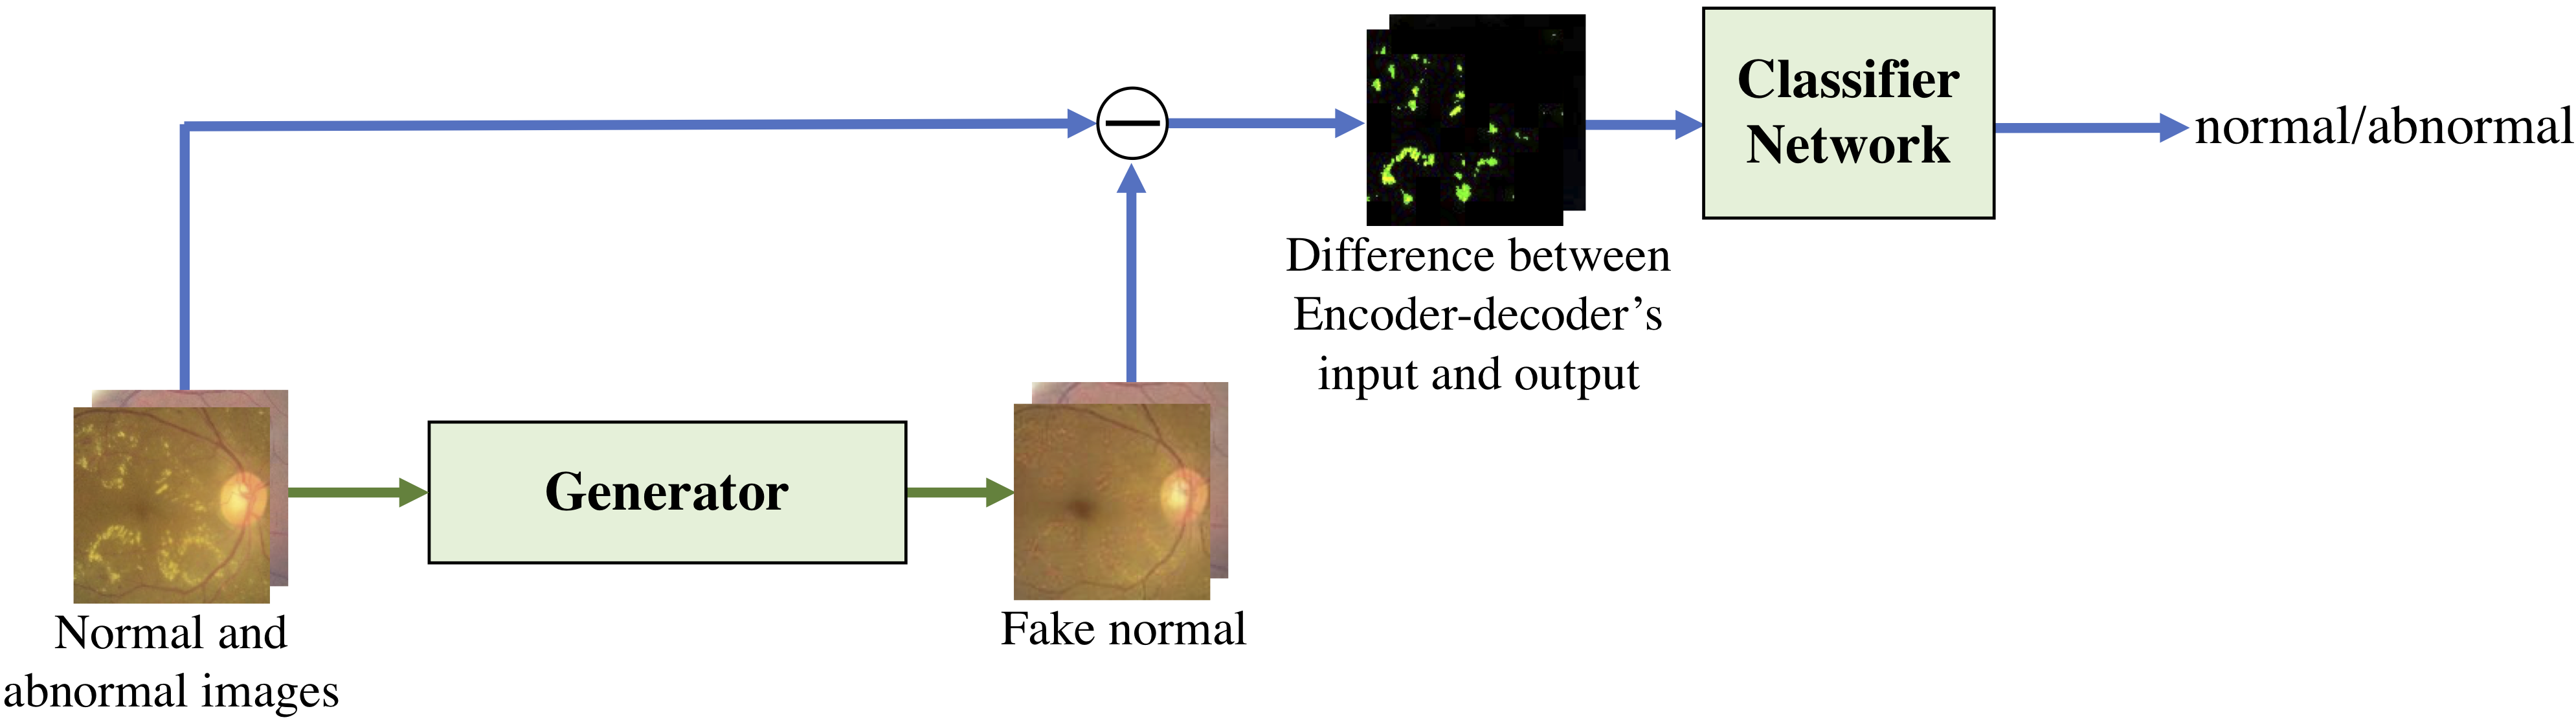
\includegraphics[width=1.0\textwidth]{figure/u_c_architecture.png}
%	\caption{同时训练编码器-解码器和CNN分类器的实际有效模型结构图。}
%	\label{fig:u_c_architecture}
%\end{figure}
%\vspace{-2cm}
%\begin{figure}[h]
%	\centering
%	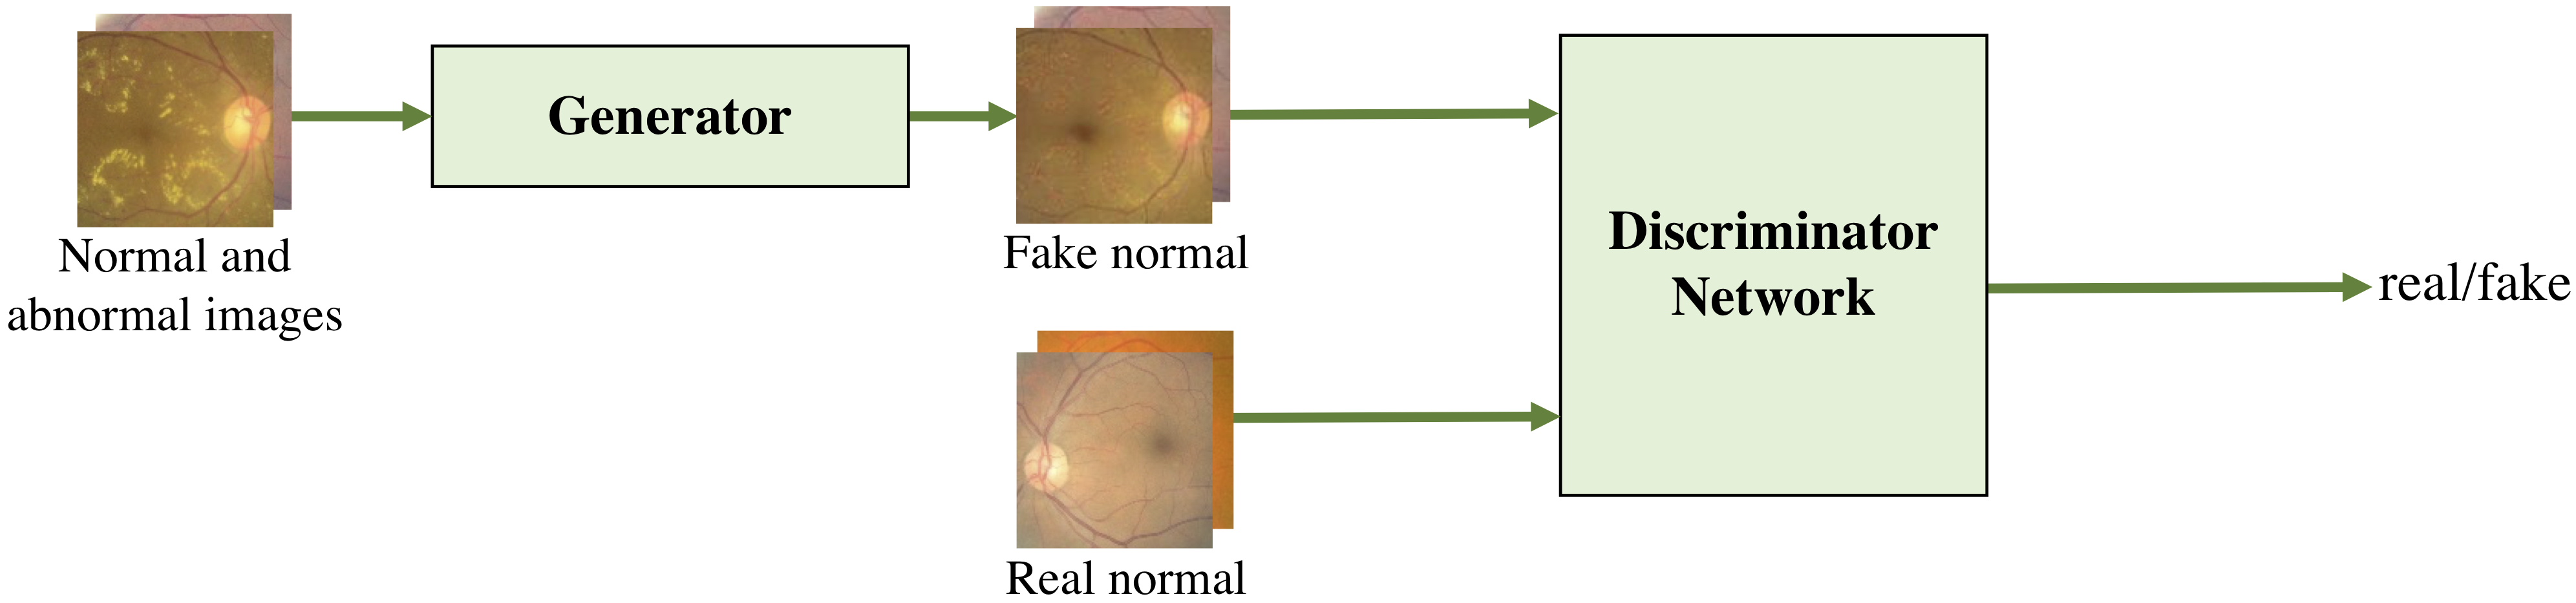
\includegraphics[width=1.0\textwidth]{figure/u_d_architecture.png}
%	\caption{同时训练编码器-解码器和判别器的实际有效模型结构图。}
%	\label{fig:u_d_architecture}
%\end{figure}
\subsection{损失函数}\label{subsec:loss_func}
接下来,本文将介绍本文模型在处理疾病标记物定位任务时的损失函数,不妨用$G$表示编码器-解码器,用$D$表示判别器,用$C$表示CNN分类器。设疾病标记物定位问题的损失函数为$\mathcal{L}$,本文将$\mathcal{L}$定义为:
\begin{equation}\label{equ:model_loss_func}
\mathcal{L}=\min _{G, C} \max _{D} \quad L_{GAN}(D, G)+\lambda_{1} L_{C E}(C, G)+\lambda_{2} L_{E D}(G).
\end{equation}
其中,$L_{GAN}(D,G)$表示对抗生成网络的损失函数(本文使用WGAN-GP),$L_{CE}(C, G)$表示CNN分类器的交叉熵损失函数,$L_{E D}(G)$是约束编码器-解码器的损失函数(本文使用L1损失函数),用于强调输入和输出之间的相似性,$\lambda{1}$和$\lambda_{2}$是两个超参数,用于平衡各个损失函数之间的权重。注意$L_{E D}(G)$这一项是不可缺少的,一旦缺少($\lambda_{2}=0$),在CNN分类器和判别器的指导下,编码器-解码器很可能在修改疾病标记物所在区域的同时还会修改正常区域,导致不可避免地出现假阳现象。

接下来,本文将给出每个步骤训练时的损失函数。根据等式\ref{equ:model_loss_func}和\ref{item:training_steps}小节中描述的训练策略,本文可进一步分别给出本文两步训练的损失函数。设第一步和第二步的损失函数分别为$L_1$和$L_2$,则第一步训练的损失函数$L_1$定义为:
\begin{equation}
\min_{G, C} \;\; L_{1}=\lambda_1 L_{CE}(C,G) + \lambda_2 L_{ED}(G).
\end{equation}
%设正常图像数据分布为$\ve{x}\sim \text{p}_{\text{n}}(\ve{x})$,异常图像数据分布为$\ve{z}\sim \text{p}_{\text{l}}(\ve{z})$,包括正常图像和异常图像在内的所有图像数据分布为$\ve{y}\sim \text{p}_{\text{all}}(\ve{y})$,分布$\text{p}_{\text{all}}$的随机取样$\ve{y}$对应的图像标签为$\ve{l}$,分布。设第一步的损失函数为$L(\ve{x};\vv{\theta})$,则第一步训练的目标是最小化损失函数$L(\ve{x};\vv{\theta})$:
%\begin{equation}
%L(\ve{x};\vv{\theta}) = \lambda_{1} %L_{CE}(G(\ve{x};\vv{\theta})-\ve{x},\ve{l}) + %\lambda_{2}L_{ED}(G(\ve{x};\vv{\theta}), \ve{x}).
%\end{equation}
第二步中训练由编码器-解码器和判别器组成的对抗生成网络,则损失函数$L_2$可定义为:
%L_{GAN}(G, D)$:
%\begin{equation}\label{equ:training_gan_loss}
%L_{GAN}(G, D)=L()=D(\ve{x};\vv{\theta})-D(G(\ve{z};\vv{\theta});\vv{\theta})+\lambda \left[\left(\left\|\nabla_{\hat{x}} D(\hat{\ve{x}};\vv{\theta})\right\|_{2}-1\right)^{2}\right].
%\end{equation}
%其中分布$p_{\hat{x}}$不是对分布$p_{all}$代表的空间采样,而只对分布$p_n$和给定分布$\text{p}_{\text{l}}$时编码器-解码器生成的图像数据分布之间的公共空间采样,$\lambda$是梯度惩罚项的权重。由于对抗生成网络的训练也是分两个阶段完成的,本文将进一步介绍每一步对应的损失函数,则训练对抗生成网络的第一步(固定$G$而更新$D$)对应的损失函数为最小化等式\ref{equ:training_gan_loss}。而第二步(固定D而更新G)对应的目标可表示为最小化损失函数${L}_{u\_d}$:
%\begin{equation*}
%	{L}_{u\_d}=-D\left(G(z)\right) + \lambda_{2}\left[L_{ED}(G(z), z) + L_{ED}(G(x), x)\right].
%\end{equation*}
\begin{equation}
\min_{G} \max_D \;\; L_{2}= L_{GAN}(D,G) + \lambda_2 L_{ED}(G).
\end{equation}

到这里,本文将模型方法相关内容叙述都已描述完毕。为了更为清晰表示其训练过程及其损失函数,与之对应的算法过程描述如算法\ref{alg:net}所示。从算法\ref{alg:net}也可以看出,本文中GAN选用的是WGAN-GP。
\begin{algorithm}[h]
	\SetAlgoLined
	\caption{本文提出的新型网络模型训练过程描述图}
	\label{alg:net}
	%\KwIn{Sample normal images $x\in \mathbb{P}_n$, lesion images $z\in \mathbb{P}_l$.}
	%\KwOut{$y$, the net activation}
	%$y\leftarrow 0$\;
	\SetKwInOut{Input}{Input}\SetKwInOut{Output}{output}
	\Input{learning rate $\alpha$, batch size $m$, hyperparameters $\lambda _1$ and $\lambda _2$, encoder-decoder's parameters $\vv{\theta} _g$, classifier's parameters $\vv{\theta} _c$, discriminator's parameters $\vv{\theta} _d$, maximum iterations $K$.}
	\nl \For{$k\leftarrow 1$ \KwTo $K$}{
		%reference: http://mlg.ulb.ac.be/files/algorithm2e.pdf
		\nl
		Sample a batch $\{\ve{x}^{(i)}\}_{i=1}^{m}$ from the normal dataset, and a batch $\{\ve{z}^{(i)}\}_{i=1}^{m}$ from the abnormal dataset; collect both to get batch $\ve{y}=\{\ve{y}^{(i)}\}_{i=1}^{2m}$, and their corresponding labels $\ve{l}=\{\ve{l}^{(i)}\}_{i=1}^{2m}$.\\
		\nl	$L(\ve{y},\ve{l};\vv{\theta})$ $\leftarrow \lambda _1$[$\frac{1}{2m}\sum_{i=1}^{2m}$$L_{CE}(C(G(\ve{y}^{(i)};\vv{\theta});\vv{\theta}), \ve{l}^{(i)})$] $+$\\
		\qquad \qquad \, \, \, $\lambda _2[\frac{1}{2m}\sum_{i=1}^{2m}L_{ED}(G(\ve{y}^{(i)};\vv{\theta}),\ve{y}^{(i)})]$  \\
		\nl	$\vv{\theta} _g$$\leftarrow Adam(\nabla _{\vv{\theta} _g} L(\ve{y},\ve{l};\vv{\theta}), \vv{\theta} _g, \alpha)$
		\tcp*{minimize G}
		\nl	$\vv{\theta} _c$$\leftarrow Adam(\nabla _{\vv{\theta} _c} L(\ve{y},\ve{l};\vv{\theta}), \vv{\theta} _c, \alpha)$
		\tcp*{minimize C}
		\nl	$\hat{\ve{x}}^{(i)}\leftarrow \eta \ve{x}^{(i)} + (1-\eta)G(\ve{z}^{(i)};\vv{\theta})$, $\eta\sim \text{U}(0, 1)$ ;\\
		
		$L(\ve{x},\hat{\ve{x}},\ve{z};\vv{\theta})$ $\leftarrow $$\frac{1}{m}\sum_{i=1}^{m}$$[D(G(\ve{z}^{(i)};\vv{\theta});\vv{\theta})-$$D(\ve{x}^{(i)};\vv{\theta})+$\\ \qquad \qquad \qquad \qquad \quad \,\, $\left(\left\|\nabla_{\hat{\ve{x}}^{(i)}} D(\hat{\ve{x}}^{(i)};\vv{\theta})\right\|_{2}-1\right)^{2}]$ \\
		\nl	$\vv{\theta} _d$$\leftarrow -Adam(\nabla _{\vv{\theta} _d} L(\ve{x},\hat{\ve{x}},\ve{z};\vv{\theta}), \vv{\theta} _d, \alpha)$ 
		\tcp*{maximize D}
		$L(\ve{x}, \ve{z}; \vv{\theta})\leftarrow -\frac{1}{m}\sum_{i=1}^{m}D(G(\ve{z}^{(i)};\vv{\theta});\vv{\theta})+\lambda_2[\frac{1}{m}\sum_{i=1}^{m}L_{ED}(G(\ve{x}^{(i)};\vv{\theta}),\ve{x}^{(i)})+$
		\\ \qquad \qquad \qquad \qquad \qquad \qquad \qquad \qquad \qquad \,
		$\frac{1}{m}\sum_{i=1}^{m}L_{ED}(G(\ve{z}^{(i)};\vv{\theta}),\ve{z}^{(i)}))]$\\
		\nl	$\vv{\theta} _g$$\leftarrow Adam(\nabla _{\vv{\theta} _g} L(\ve{x}, \ve{z}; \vv{\theta}), \vv{\theta} _g, \alpha)$ 
		\tcp*{minimize G}
	}
\end{algorithm}
\section{本章小结}\label{sec:chapter3_summary}
本章内容主要围绕介绍本文提出的模型方法结构而展开。首先在\ref{sec:idea_thinking}小节介绍了本文提出新型方法的背后思考、相关模型分析以及引入各个子模块的必要性和重要性。简单来说,本文提出的模型共包括三个子模块:编码器-解码器、CNN分类器和判别器。该模型以编码器-解码器为骨架网络,以CNN分类器和判别器为辅助角色来指导编码器-解码器,使其具备识别疾病标记物的能力。另外,编码器-解码器和判别器组成了对抗生成网络。与传统的CAM和Grad-CAM等方法不同的是,本文从图像生成的角度来完成疾病标记物精确定位任务,给定任意一张输入图像,希望通过CNN分类器给出其类别(正常/异常),如果是异常,通过编码器-解码器的输出和输入之差来给出疾病标记物的精确位置。随后,本文在\ref{sec:model_architecture_intro}小节给出模型结构图,并详细介绍了三个子模块的模型结构示意图(相关内容参见\ref{subsec:encoder_decoder_model}小节、\ref{subsec:cnn_classifier_model}小节和\ref{subsec:discrimintor_model}小节),以期读者不仅能对本文提出的模型有宏观上的理解,还不缺对各个子模块细节上的详实说明。最后,本文在\ref{sec:loss_func_training_stragies}小节中给出了模型训练的两步训练策略(见\ref{item:training_steps}小节)和模型训练的损失函数(见等式\ref{equ:model_loss_func})。为了方便读者进一步理解本文提出的训练策略,在算法\ref{alg:net}中,本文还用形式化语言描述了模型训练过程以及每一步的损失函数。到此,本文提出的模型方法的相关介绍结束,接下来将在第\ref{sec:experiments}章和第\ref{sec:multi_classes}章中介绍相关实验。

